%\section{Hetergeneous Access Point Band Selection}
%\label{sec:moa_problemformulation}
%
%% Introduce the content of this section
%In this section, we illustrate the challenges of hetergenous access point 
%band selection in wireless network deployment and formulate the problem of band 
%selection in mesh network deployments jointly using WiFi and white space bands. 
%Further, we present a linear program and MHAPD(Multiband Hetergeneous AP Deployment) algorithm for estimating the 
%access point number to serve the traffic demand of a given population.
%Then we discuss the application of the algorithm in uniform population
%distribution and non-uniform population distribution with spectrum resource 
%variation to tell the general rules in picking up channels for access points.
 
%\subsection{White Space Opportunity and Challenge}
%\label{subsec:motivation}

%% Propagation
%Wireless propagation is the behavior of the signal loss characteristics 
%when wireless signals are transmitted through the wireless medium.
%The strength of the received signal depends on both the line-of-sight
%path (or lack thereof) and multiple other paths that result from 
%reflection, diffraction, and scattering from 
%obstacles~\cite{andersen1995propagation}. The widely-used Friis
%equation characterizes the received signal power $P_r$ in terms 
%of transmit power $P_t$, transmitter gain $G_t$, receiver gain $G_r$, 
%wavelength $\lambda$ of the carrier frequency, 
%distance $R$ from transmitter to receiver, and path loss exponent 
%$n$ according to~\cite{friis}:
%\begin{equation}
%\label{eq:friis}
%P_r=P_t+G_t+G_r+10n \log_{10}\left( \frac{\lambda}{4\pi R}\right)
%\end{equation}
%Here, $n$ varies according to the aforementioned environmental 
%factors with the value of two to five in typical outdoor 
%settings~\cite{rappaport}.

% Hetergenous access points
%Despite sufficient levels of received signal, interference can cause channels
%to be unusable (e.g., due to high levels of packet loss) or unavailable (e.g.,
%due to primary users in cognitive radios~\cite{haykin2005cognitive}).
%Prior work has worked to reduce cost through gateway deployment, channel 
%assignment, and routing~\cite{he2008optimizing,tang2005interference}.
%Most of existing works try to reduce the intra-network interference or increase
%the channel usability level of wireless network deployment
%~\cite{si2010overview,joshi2009efficient}. However, the access point service area
%variation becomes an important problem when considering the availability of white space bands.  
%Jointly considering the propagation and single channel capacity, the access points 
%with different configuration (e.g. radios) in the same area, or with same configuration 
%in diverse population density areas (e.g. downtown, rural) could have different service ranges.
%
%% Explain multiband and hetergenous access points
%When wireless devices operate in WiFi bands, the channel separation is relatively
%small (e.g., 22 MHz for the 2.4 GHz band). As a result, many works assume that
%the propagation characteristics across channels are similar. However, with the
%large frequency gaps of WiFi and white space bands (e.g., several GHz),
%propagation becomes a key factor in the deployment of wireless networks with both bands.
%Here, a frequency band is defined as a group of channels which have
%small separation meaning similar propagation characteristics.
%In this work, we consider the diverse propagation and activity characteristics
%for four total frequency bands: 450 MHz, 800 MHz, 2.4 GHz, and 5.2 GHz.
%We refer to the two former frequency bands as white space bands and
%the two latter frequency bands as WiFi bands.
%A general way to increase the capacity of a single access point is to add channels
%through radios~\cite{raniwala2005architecture}. The assumption all the channels have
%the same propagation does not fit for WiFi and white space hetergenous scenario.
%When a white space band channel added to an access point, the capacity and service 
%range could increase simultaneously. The differences in propagation and constraints 
%of network deployment create opportunity for the joint use of white space and 
%WiFi bands in wireless access networks according to the environmental characteristics 
%(e.g., urban or rural and downtown or residential) of the deployment location.
%
%% Network Constraints
%Typically, the deployment of wireless access networks is subject to coverage and capacity
%constraints for a given region. Coverage is defined with respect to the ability of
%clients to connect to access points within their service area.  We use a coverage
%constraint ratio of $95\%$ in this work for a target area~\cite{robinson2010deploying}.
%Capacity is defined with respect to the ability of a network to serve the traffic 
%demand of clients.  Spatial reuse allows improved capacity, but increases the cost
%of deploying a network by increasing the total number of access points required.
%Hence, for densely populated areas the greatest level of spatial reuse possible
%is often desired. And the deployment cost could be significant reduced through access 
%points with high capacity with more centralized using radios. In contrast, 
%sparsely-populated rural areas have lower traffic demand per unit area. Thus, 
%aggregating this demand with lower-frequency, white space bands could be highly 
%effective in reducing the total number of access points required to achieve 
%similar coverage and capacity constraints. Moreover, since less TV channels tend
% to be occupied in sparsely populated areas~\cite{msdatabase}, a larger number 
% of white space bands can be leveraged in these areas. 

% More variation in population distribution



\section{Heterogeneous Access Point Band Selection}
\label{subsec:moaproblem}

% Assumptions of the network
As opposed to previous works such as ~\cite{franklin2007node,robinson2010deploying,si2010overview}, 
this work focus on heterogeneous access point band selection for wireless access networks which jointly employ WiFi 
and white space bands. We propose a relaxed linear program to find the lower bound of the number of access points
and a Multiband Heterogeneous Access Point Deployment (MHAPD) algorithm  to approach the lower bound 
number of access points which serve the traffic demand of a certain area. We assume the network carrier has a limited number 
of spectrum resources and radios have similar configurations in terms of transmission power and bandwidth per channel use. 
Each radio on an access point operates with a classic protocol model as introduced in~\cite{gupta2000capacity}. 
We further assume that there is a given take rate and traffic demand for a given population (as specified in Section
~\ref{sec:moaexperimentdesign}).

%% Capacity constraint
%A network deployment should ideally provide network capacity equal to the demand of the service 
%area to maintain the capacity constraint. The demand of a service area could be calculated as the 
%summation of individual demands all over the service area $D_a=\sum_{p\in P}D_p$. Since 
%household demand for Internet has been previously characterized~\cite{rosston2011household}, 
%$D_a$ could represent the population distribution $f$ and service area $k$ as 
%$D_a=\sum_{f \in F,k \in K}\bar{D_p}*f*k$. 
%The capacity constraint could be represented with access points set $M$ according to:
%\begin{equation}
%\label{eq:nlbound}
%\sum_{m \in M}C_r^m \ge \sum_{f \in F,k \in K}\bar{D_p}*f*k
%\end{equation}
%% Coverage constraint
%At the same time, the wireless network must additionally satisfy the coverage constraint in the service 
%area where the access points provide connectivity for client devices. 
%Generally, a coverage of $95\%$ is acceptable for wireless access networks~\cite{robinson2010deploying}.
%The object of this work is to find the best possible number of access points so that the network has good 
%connectivity and enough capacity to satisfy the traffic demands.


% Hetergeneous Access point & resource constraint
Under the capacity and coverage constraints, the service area of a heterogeneous multiband access point deployments
varies according to the users' traffic demand. The service area is limited by the propagation range when the traffic 
demand is low. Conversely when the traffic demand is high, the service area is limited by the radio capacity.The 
radius of the service area $r_s$ could be represented as Eq.~\ref{eq:servicearea}:
\begin{equation}
\label{eq:servicearea}
r_s=min\{r_p,r_c\}
\end{equation}

Here, $r_p$ represents the propagation range of a radio in the access point, and $r_c$ is the capacity range of 
the radios in the access point. When the traffic demand is distributed uniformly in a circle, from Eq.
~\ref{eq:nlbound} the capacity range $r_c$ could be denoted as $r_c=\sqrt{k/\pi}$. Moreover, the propagation 
range and capacity range could be determined by the environment, traffic distribution, and transmission power 
control~\cite{robinson2010deploying}. These factors are out of the scope of this work, but they could easily 
be added to the model for calculation of the heterogeneous access point service area. To simplify the problem 
and focus on the role of multiple frequency bands, we assume the traffic demand is uniformly distributed and 
the propagation follows Friis rule as Eq.~\ref{eq:friis}. When the input target area and the census parameters 
are given, we could obtain the service area of each access point type through~\ref{eq:servicearea}. To increase 
the spatial reuse in practice, we then adjust the transmit power of each radio to reduce the interference if 
the service area is limited by the radio capacity since we adopt the protocol model. 
% Variation of radios
For example, if we assume all the access points have the same number of radios and channel resources,
%When the target area is given, thre traffic demand of the area could be calculated through the parameters, 
%the service area of a heterogeneous access point varies with the radios due to the constraints. 
% Lower traffic demand case
in a low traffic demand scenario, the service radius reaches the radio propagation range. A high frequency 
WiFi radio will have a smaller service area since the signal attenuate faster; while the white space radio 
could have a larger service area due to the longer propagation range; and a heterogeneous access point who 
has both WiFi radios and white space radios has the same range of as low frequency radios access point. 
The example is shown in Fig.~\ref{fig:lowtraffic}.
% Medium traffic demand case
In a medium traffic demand scenario, heterogeneous access points and white space access points will 
have the same size service area which is larger than high frequency WiFi only access points as shown in Fig.
~\ref{fig:mediumtraffic}.
% High traffic demand case
With high traffic demand, all access points will have the same service area due to capacity constraint 
as shown in Fig.~\ref{fig:hightraffic}. White space bands could reduce the cost of wireless network 
deployment due to greater inter node spacing and channel resources. 
Thus, lowest cost for covering a certain area is to use white space bands in all access points 
if the traffic demand and user density is sufficient. 
%based on the analysis.
However, spectrum resources are limited and the use of white space bands are restricted in major 
cities in the US due to TV channel occupancy~\cite{msdatabase}. 
% Problem
Thus, the tradeoff between centralized use of white space bands or mixed use of white space
bands and WiFi bands under multiple traffic demands is question for wireless network deployment. 
The problem could be modeled as how to use the minimum number of multiple sizes of service area according to 
radio combinations to cover a certain 2-D plane. This problem is to deploy different size of cells in 
a given plane, which is a NP-hard bin packing problem~\cite{martello1998exact}. 
To achieve the lower bound number of access points, We propose a relaxed linear program and a 
heuristic algorithm to approach the lower bound.



\begin{figure}
%\vspace{-0.0in}
\centering
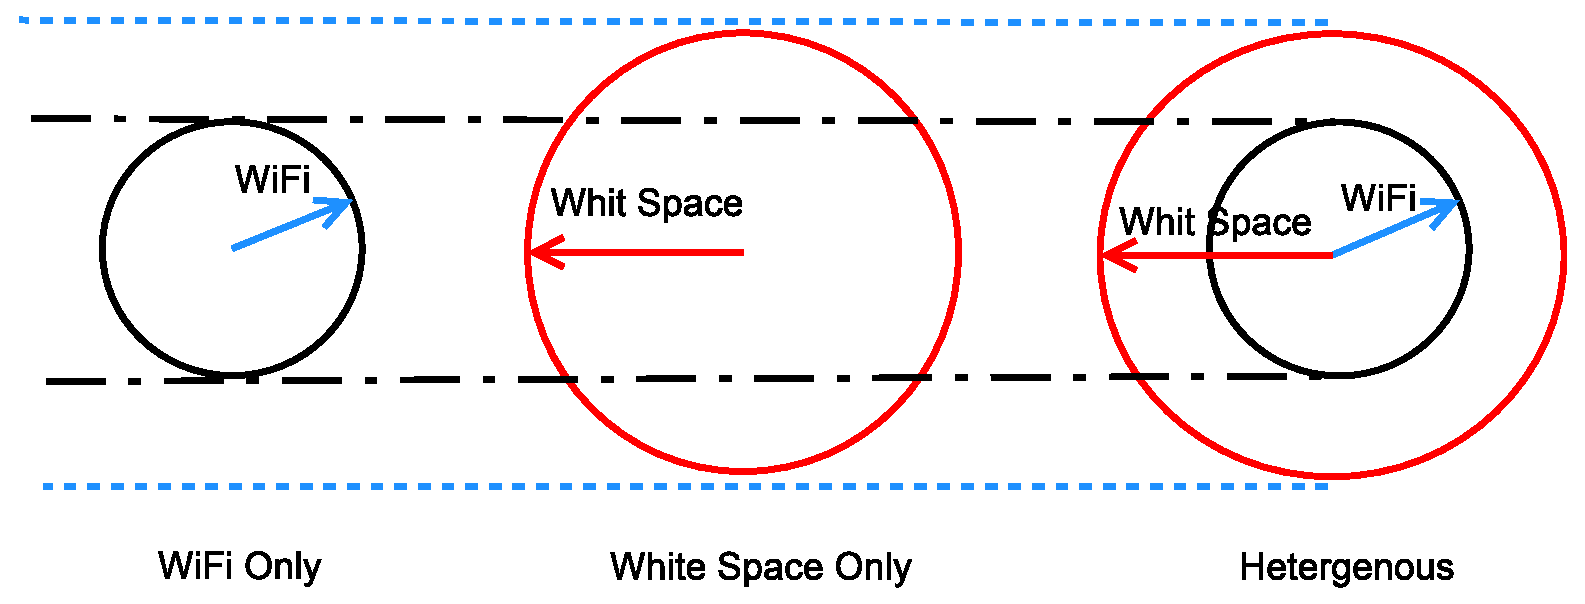
\includegraphics[width=84mm]{figures/lowtraffic}
\vspace{-0.1in}
\caption{Low Traffic Scenario}                                                                 
\label{fig:lowtraffic}
%\vspace{-0.1in}
%\end{figure}

%\begin{figure}[H]
%\vspace{-0.0in}
%\centering
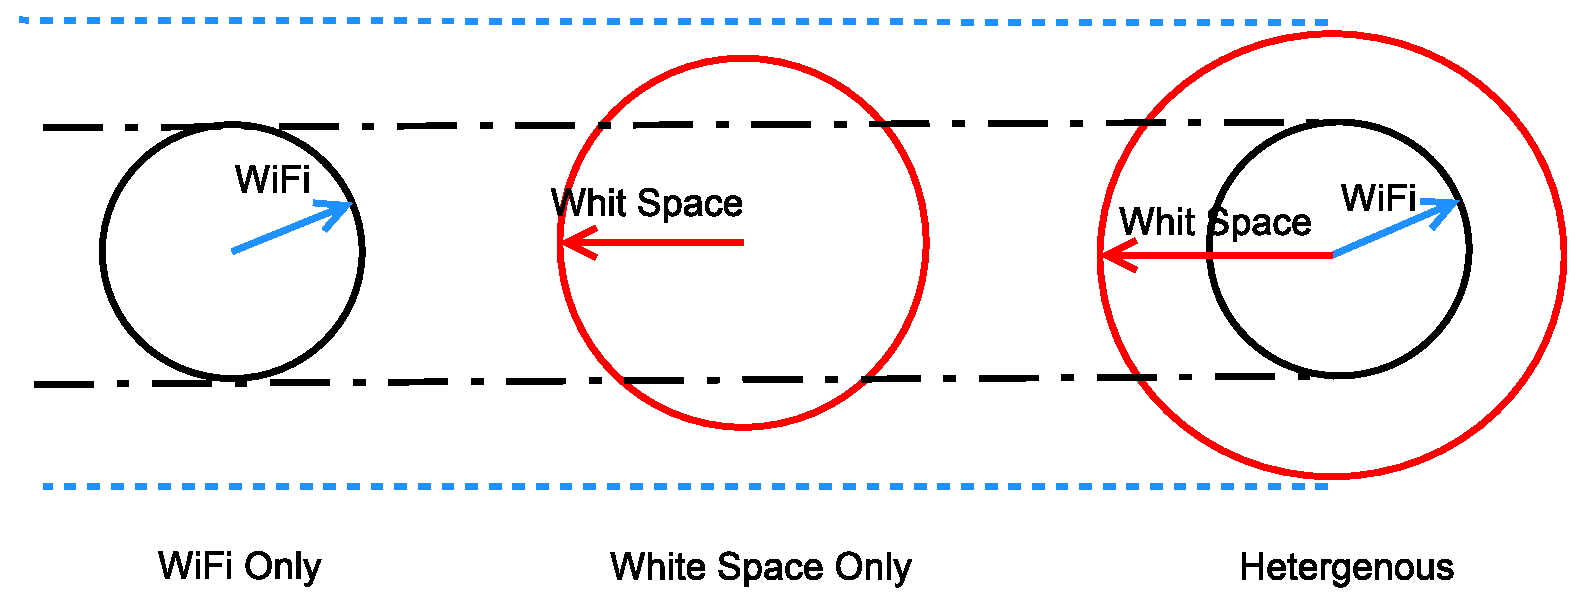
\includegraphics[width=84mm]{figures/mediumtraffic}
\vspace{-0.1in}
\caption{Medium Traffic Scenario}                                                                 
\label{fig:mediumtraffic}
%\vspace{-0.1in}
%\end{figure}


%\begin{figure}[H]
%\vspace{-0.0in}
%\centering
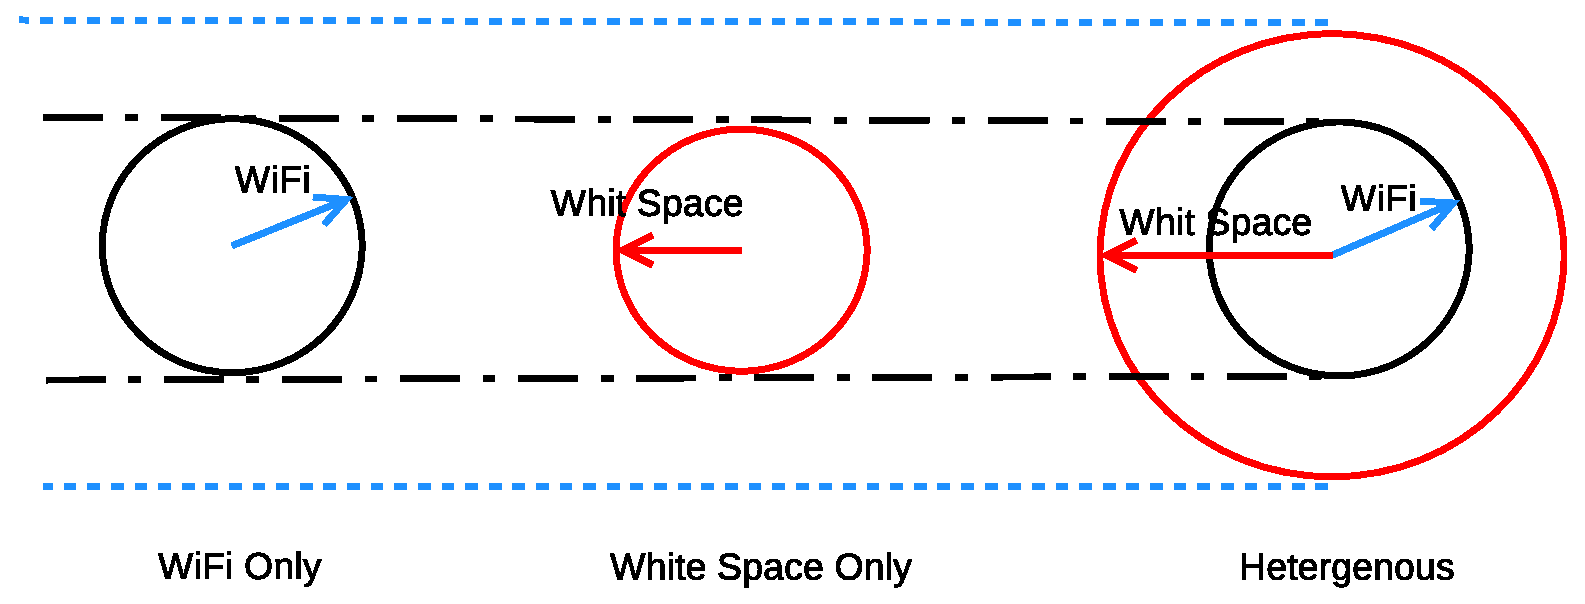
\includegraphics[width=84mm]{figures/hightraffic}
\vspace{-0.1in}
\caption{High Traffic Scenario}                                                                 
\label{fig:hightraffic}
\vspace{-0.1in}
\end{figure}

% Relaxed linear program
The input of the problem include a given target area $G$ with the traffic demand distribution $\gamma$, 
the service area of all kinds access points $S_t$, and the coverage rate $p$, then the capacity of access 
point $C_t$ could be calculated based on the number of radios, Friis model in Eq.~\ref{eq:friis} 
and restriction constraints in Eq.~\ref{eq:servicearea} or from in-field measurement~\cite{cuileveraging}. 
When the target area is served, the reward of the area denoted as $R$ could be calculated. 
A network carrier is supposed to cover the whole target area with a constant percent, so that the reward 
of the carrier from charging the users in the target area is constant. Thus, to maximum the profit, 
reducing the cost of building the access points is the key part of the network
carrier. 

We introduce our linear program approaching as follows:

\noindent
{\bf Sets:}
\begin{tabular}{ll}
$B$ & Set of Bands \\
$T$ & Type of Access Point\\
\end{tabular}

\noindent
{\bf Parameters:}\\
\\
%\vspace{0.1in}
%\begin{tabular}{lll}
\begin{tabular}{llp{3.4cm}}
$G$ &  & Target Area\\
$\gamma$ & & Traffic Demand Distribution\\
$p$ & & Coverage Rate\\
$S_t$ & $t \in T$ & Coverage Area of Type t AP\\
$O_{b,t}$ & $b \in B, t \in T\ binary$ & Channel Occupied by Type t AP\\
$N_b$ & $b \in B\ $ & Available channel of a band in Target Area\\
$C_t$ & $t \in T$ & Channel capacity of Type t AP\\
\end{tabular}


\noindent
%\vspace{2pt}
{\bf Variables:}\\
\\
%\vspace{1pt}
\begin{tabular}{llr}
$a_t\ge0$ & $t \in T$ & Number of Type t AP\\ 
\end{tabular}

\noindent
{\bf Objective:}
\begin{align}
& Min \sum_t a_t
\end{align}

\noindent
%{\bf Constraints:}
{\bf Coverage Constraint:}
\begin{align}
\label{opt:coverage}
\sum_t a_t\cdot S_t \ge G*p
\end{align}
\noindent
{\bf Capacity Constraint:} 
\begin{align}
\label{opt:capacity}
\sum_t a_t\cdot C_t \ge G\cdot \gamma
\end{align}
\noindent
{\bf Resource Constraint:} 
\begin{align}
\label{opt:resource}
\sum_t a_t\cdot O_{b,t} \le N_b
\end{align}

{\bf Spatial Constraint:} 
\begin{align}
\label{opt:resource}
a_t < \frac{G}{S_t}\cdot\frac{2}{3}\cdot N_b
\end{align}


The linear program relaxes the coverage constraint without providing a key parameter where the access 
points are located. Moreover, the linear program may provide multiple results since different types of 
access points could have the same service area (e.g. in a low traffic demand case). The result of the 
linear program is the lower bound on the number of access points. 

In order to find a practical access points deployment in multiband scenario, we represent 
a greedy local search algorithm in Alg.~\ref{alg:gls}. The service area of access points varies 
across diverse population distributions. Assume the cost of building an access point is the same as $C_a$. 
When an access point is built, the more service area the better. Thus, heterogeneous access points
could always have better performance. However, since there are a limited spectrum resources,
we have to balance the usability of heterogeneous access points which reduce the cost of building 
a network, and single radio access point which may cover more area.

In the linear program, the reward $R$ is a constant of the area $G$. But for a single heterogeneous 
access point deployment, we have to compare its reward and cost to separately using the radios. In a 
certain area, a heterogeneous AP has radius $r_1$. If we separately use the radios with radius $r_2,r_3,\dots r_n$, 
the reward is uniformly distributed and the heterogeneous reward is defined as:

\begin{equation}
\label{eq:unitprice}
H_r=(n-1) C_a - \frac{R}{G}\cdot\sum f_s(r_n)
\end{equation}

Here, $f_s(r)$ is the area calculated function, for example, $f_s = \frac{3\sqrt{3}}{2}r^2$ when a 
hexagonal coverage model is applied. In the framework, the access point type with greater reward 
is going to deployed first until the available resources are used up. When two types of access points
share the same unit price, considering the spatial reuse, the access points with high frequency channels
will be chosen. The deployment starts from the edge of the given plane and we use a protocol model
to find the available access point types. If the combination of a unit grid could be covered by an 
access point, we put the unit grid in the coverage area until the access point can not access any 
more of grid. Then we switch to another available access point. The process is like a Teris game, 
when a given access point is filled, it will be deleted.
% Algorithm for lower bound approaching
\begin{algorithm}
\caption{Multiband Heterogeneous AP Deployment}
\label{alg:gls}
\begin{algorithmic}[1]
\REQUIRE  ~~\\
$G$: Target Area \\
$R$: Reward of Target Area \\
$\gamma$: Traffic Demand Distribution\\
$p$: Coverage Rate\\
$S_t$: Coverage Area of Type t AP \\
$O_{b,t}$: Channel Occupied by t Type AP\\
$N_b$: Available channels of a Band in Target Area\\
$C_t$: Channel Capacity of Type t AP
\WHILE {$\sum A\cdot S_t < p$}
\STATE Rank available AP type according to their unit price $H_r$
\STATE Rank available AP type according to radio numbers
\IF {The reminder area $G_r$ is larger than all the available AP}
\STATE Choose the AP has the largest coverage area $S_t$
\ELSE 
\STATE Find the available AP type whose coverage area $S_t=min{S_t>G_r}$
\ENDIF
\STATE Deploy an AP at the left up edge of un-covered area
\STATE Fill the AP with one neighbor unit grid and move the AP in the center of the coverage area
\STATE Update Channel Resource $O_{b,t}, N_b$
\STATE Update Output Access Point $A$
\ENDWHILE
\ENSURE ~~\\
The number of Access Points and Deployment\\
\end{algorithmic}
\end{algorithm}
% Algorithm analysis and justify

Generally, we employ access points with larger coverage capacity to fill in the area. Then 
through the algorithm, we could cover the target area by the most efficient access point type,
step by step until a  minimum number of access points and a practical multiband wireless 
deployment is achieved.
